\documentclass[journal]{IEEEtran} % use the `journal` option for ITherm conference style
\IEEEoverridecommandlockouts
% The preceding line is only needed to identify funding in the first footnote. If that is unneeded, please comment it out.

\usepackage{hyperref}
\usepackage{cite}
\usepackage{amsmath,amssymb,amsfonts}
\usepackage{algorithmic}
\usepackage{graphicx}
\usepackage{textcomp}
\usepackage{xcolor}
\usepackage{graphicx} % To include images
\usepackage{float} % To use [H] for figure placement
\graphicspath{{img/}}

\def\BibTeX{{\rm B\kern-.05em{\sc i\kern-.025em b}\kern-.08em
    T\kern-.1667em\lower.7ex\hbox{E}\kern-.125emX}}

\begin{document}

\title{Enhanced Spectrum Sensing Techniques For 5G New Radio (NR) And Long-Term Evolution (LTE) Utilizing Unet-Based Deep Learning Network\\
% delete or comment-out the following line before submission
% {\footnotesize \textsuperscript{*}Note: Sub-titles are not captured in Xplore and should not be used}
% \thanks{Identify applicable funding agency here. If none, delete this.}
}

\author{%%%% author names
    \IEEEauthorblockN{\textsuperscript{1} Huan Nguyen-Duy}% first author
    , \IEEEauthorblockN{\textsuperscript{2} Dr.Thien Huynh-The}% delete this line if not needed
    %, \IEEEauthorblockN{\textsuperscript{} who ?}% delete this line if not needed
    % duplicate the line above as many times as needed to list all authors
    \\%%%% author affiliations
    \IEEEauthorblockA{\textsuperscript{1, 2}\textit{Ho Chi Minh City University of Technology and Education (HCMUTE), Vietnam}}\\% first affiliation
    \IEEEauthorblockA{\textsuperscript{1, 2}\textit{The Intelligent Multimedia and Advanced Computing (IMAC) Laboratory}}\\% delete this line if not needed
    % duplicate the line above as many times as needed to list all affiliations
    %%%% corresponding author contact details
    \IEEEauthorblockA{\textsuperscript{1}huan2931@gmail.com} \\
    \IEEEauthorblockA{\textsuperscript{2}thienht@hcmute.edu.vn}
}

\maketitle

\begin{abstract}
Spectrum sensing has a crucial role in the next generation new radio and long-term evolution network, allowing devices to identify and accommodating demand for wireless connectivity. In this paper, we address spectrum sensing challenges and introduce a innovative wireless communication network called WiComNet to tackle over-the-air communication sensing tasks. In our proposed network, which employs an architecture based on Unet, we integrate several advanced deep learning methodologies aimed at enhancing sensing performance. These include depthwise separable convolution, recurrent residual block, and atrous spatial pyramid pooling techniques, among others. Relying on simulation result, WiComNet acquired synthetic signal dataset of two wireless communication types in differenct signal-to-noise, our proposed outperformed a impressive result with high performance for spectrum sensing mission. Our implementation and pre-trained model are available at:
    \href{https://github.com/Winxkin/Spectrum_sensing_base_on_Deep_learning.git}{Spectrum sensing base on deep learning Github project}
\end{abstract}

\begin{IEEEkeywords}
    wireless communication network (WiComNet), spectrum sensing, 5G New Radio (5G NR), Long-Term Evolution (LTE), Unet, semantic image segmentation, signal processing.
\end{IEEEkeywords}

\section{Introduction}

\subsection{Spectrum sensing}
Spectrum sensing is defined as identifying the availability and non-availability of wireless communication network or radio network in a particular frequency band. When frequency allocation scheme cannot provide high data rate demand constantly, it leads to waste spectrum resources that can utilize to allocate for others such 5G new radio (NR) or long-term evolution (LTE) in the same time. Therefore, spectrum sensing for 5G NR and LTE became a main topic that have many challenges, addressing the research direction to increase effectiveness performance and utilizing limited spectrum resource. Figure 1 show the example of spectrum sensing for 5G and LTE application.

\begin{figure}[h]
    \centering
    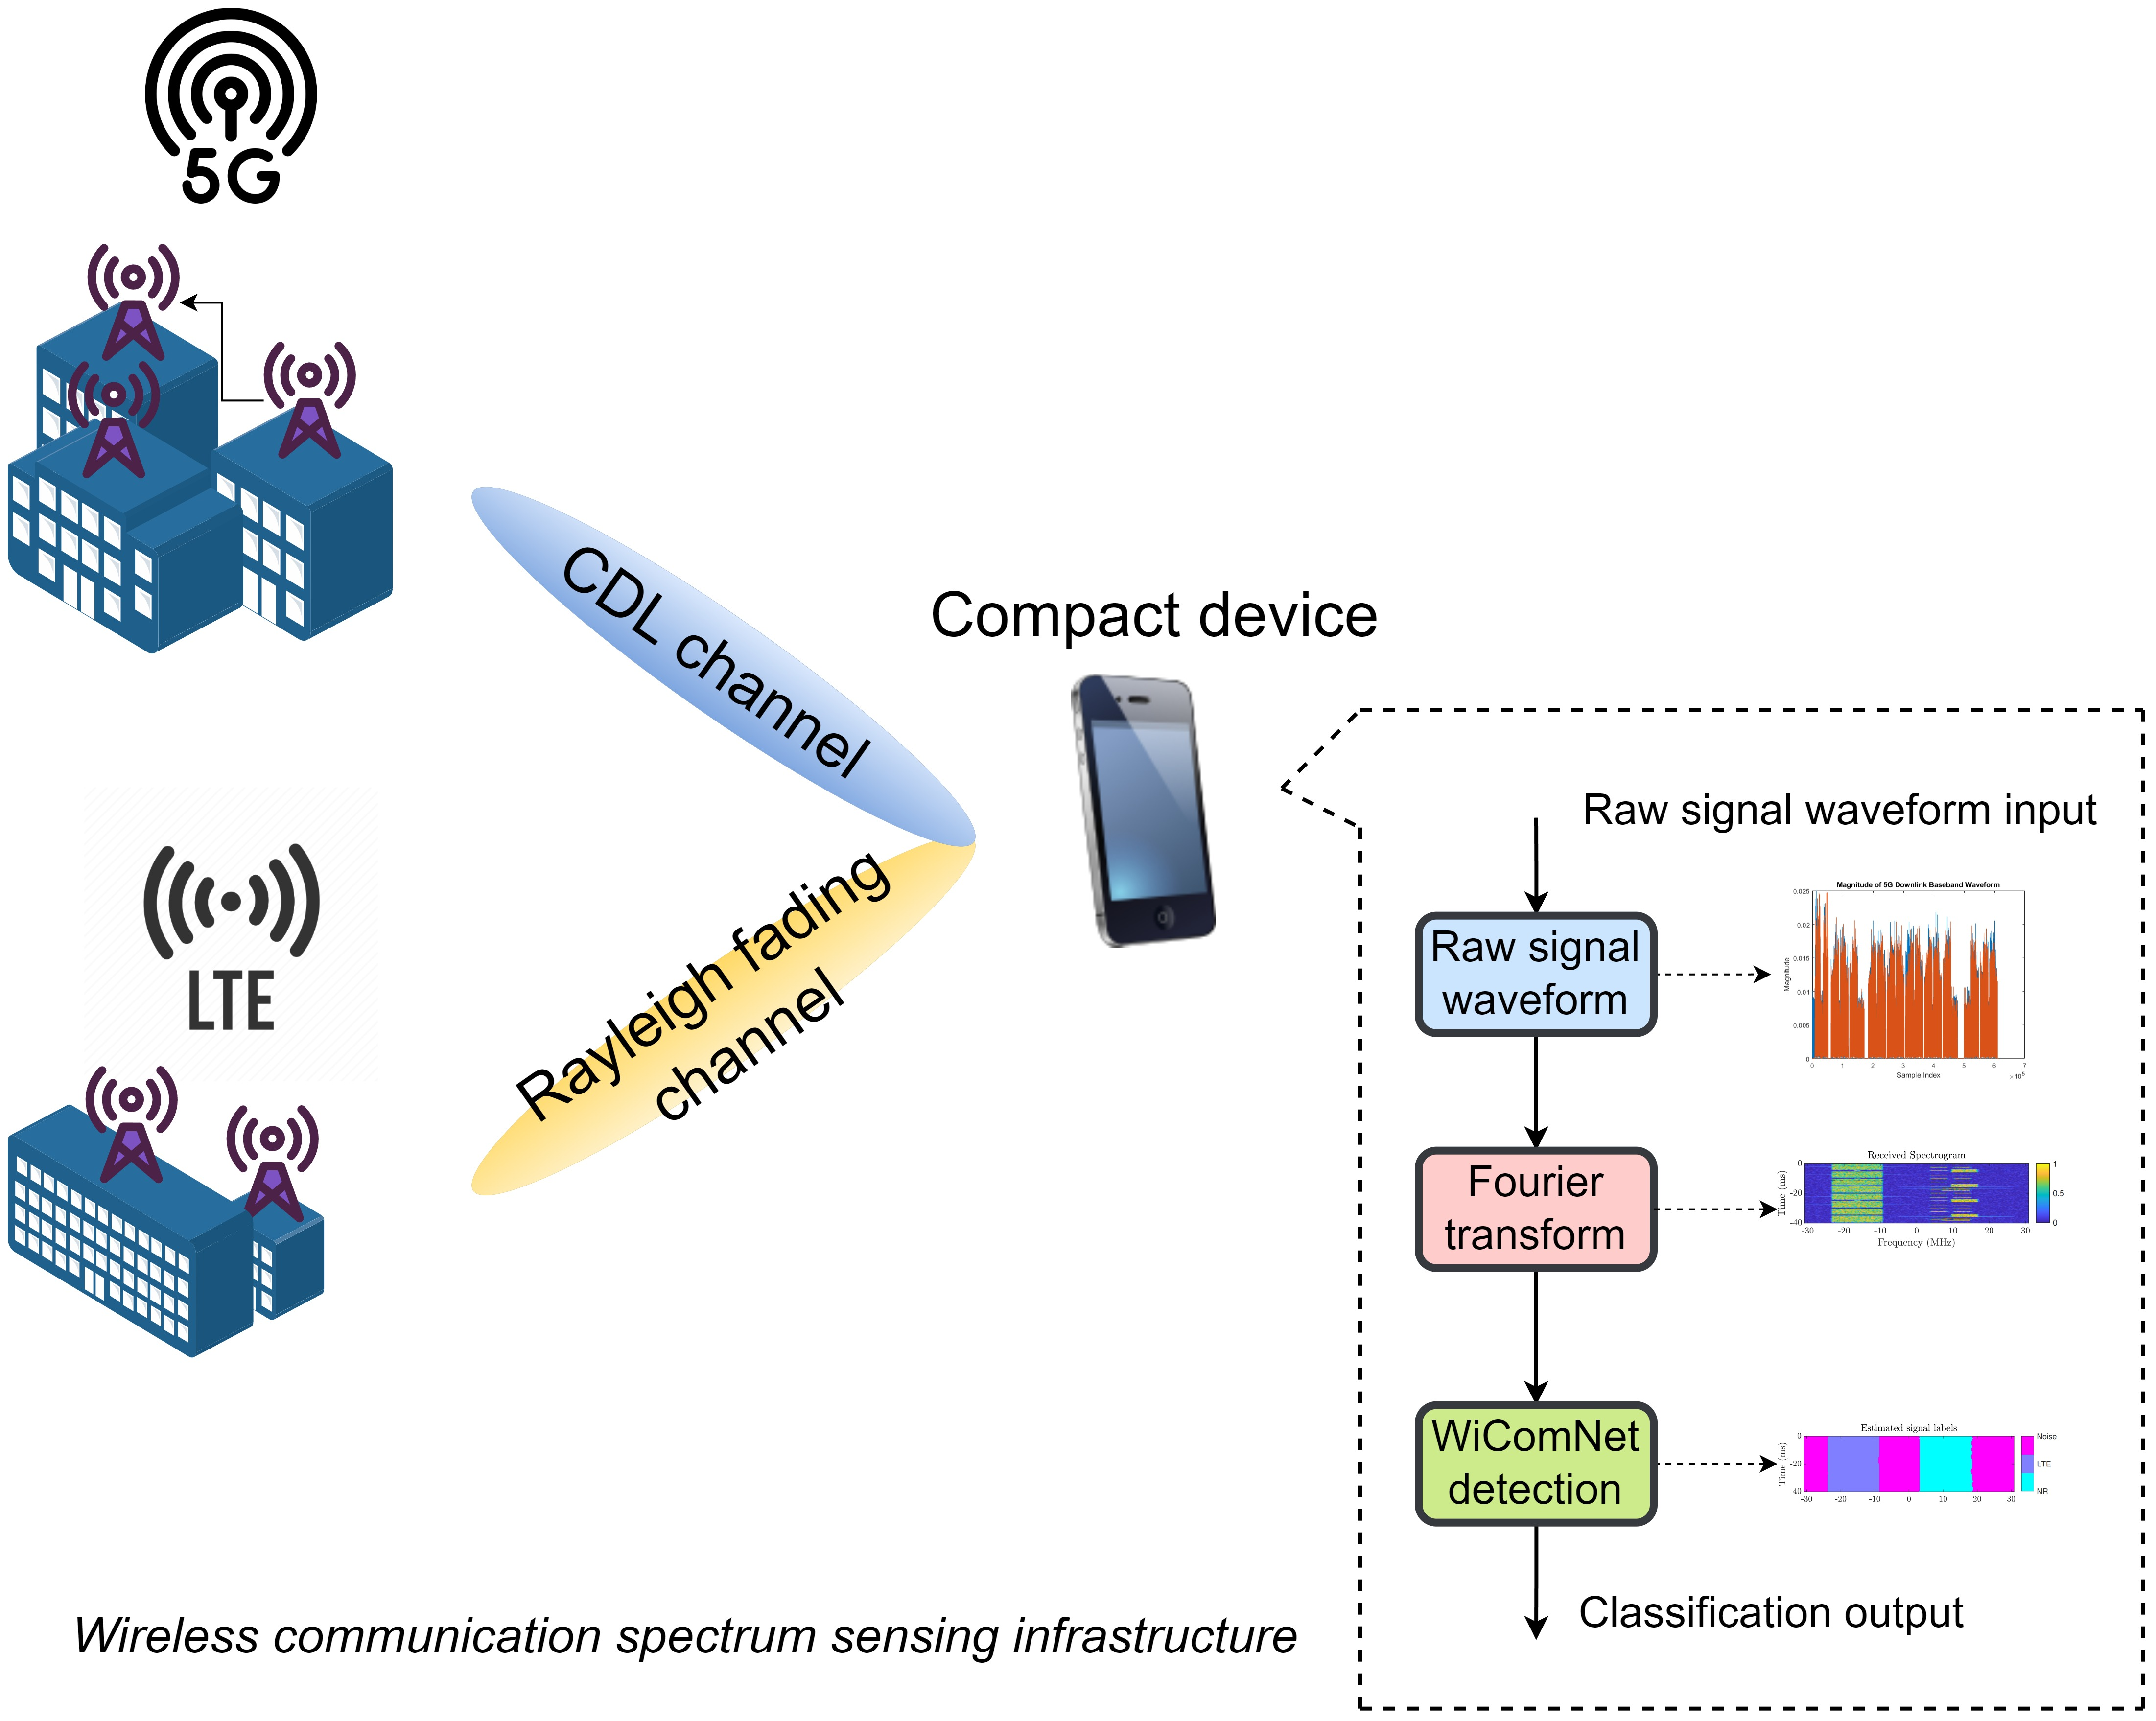
\includegraphics[width=0.35\textwidth]{img/Design-Overview.jpg}
    \caption{Spectrum sensing for 5G and LTE application.}
    \label{fig1}
\end{figure}

\\
\indent 
In the past, numerous sensing techniques were showed in \cite{YucekSpectrumSensing}, using sensing algorithms, Multi-Dimensional spectrum sensing, channel estimation, and cooperative sensing. Nevertheless, spectrum sensing task met a big challenging in hardware requirements \cite{YucekSpectrumSensing}, this task requires high sampling rates, high resolution analog to digital converters (ADC) with large dynamic range, and high performance of processor. On the other hand, Cognitive wireless communication can be identified immediately by sensing duration and frequency. However, this method trades off between performance and sensing algorithms. Since their introduction, researches spent efforts to tackle improved spectrum sensing problems, addressing various challenges and introducing innovative solutions to increase prediction ratio and performance in cognitive wireless communication network. Furthermore, prominent surveys on this topic were introduced in \cite{kumar2024analysis}, \cite{YucekSpectrumSensing}, \cite{ali2016advances}, and \cite{liyanaarachchi2021optimized}.


\subsection{Related work}
In recent years, many works on cognitive wireless communication and radio network  were introduced to enhance sensing performance. In general, energy detector based sensing is common way of spectrum sensing because it offers low computational and implementation complexities, waveform base sensing increases sensing performance, cyclostationarity based sensing for detecting and matching filtering  primary user transmissions \cite{YucekSpectrumSensing}. On the other hand, several innovative deep learning (DL) methods were presented to tackle spectrum sensing performance. Applying convolution neural network for improved waveform classification \cite{huynh2024improved}, the work \cite{huynhthe2023intelligence} introduced innovative DL architecture to improve the spectrum sensing prediction ratio for 5G and LTE signals. Other works utilized deeplabv3+ \cite{nguyen2023accurate} and DetectNet \cite{gao2019deep} to increase accuracy for spectrum sensing task. Nevertheless, while sensing algorithms have a trades-off between hardware performance and computation complexities, DL models offer higher parameters to reach a high level of precision that requires considerable hardware resources.

\subsection{Contribution}
In this work, we utilize DL methods to tackle sensing tasks and propose a innovative DL architecture based on Unet called wireless communication network (WiComNet), which reduces significantly complexity and enhances sensing performance for 5G and LTE signals. Unet was a fully convolutional network \cite{ronneberger2015u} using special for semantic segmentation images, it was designed with parallel encoder-decoder and connecting each layer by skip connection. Furthermore, Unetpp and other variant models were showed by the authors \cite{zhou2019unet++} that improve dramatically prediction ratio for image segmentation tasks. Nevertheless, the drawback of these models is that they offer significantly complexities and require considerable hardware resources. In term of decreasing complexities, we presented a WiComNet architecture that incorporated depthwise separable convolution \cite{CholletXception} and recurrent residual convolution \cite{AlomNuclei} \cite{he2016deep} \cite{aghalari2021brain}, replacing for Unet blocks in each layer of encoder and decoder paths. On the other hand, atrous pyramid spatial pooling modules \cite{ChenAtrous} were adapted between encoder and decoder paths that enhanced features extraction in multiple scales. In summary, we make the following two main contributions:
\begin{itemize}
\item[1.] Addressing spectrum sensing for 5G and LTE problems and utilizing DL methods to tackle spectrum sensing tasks.
\item[2.] Introduction a innovative WiComNet architecture based on Unet that reduces significant complexities and enhances sensing performance for 5G and LTE signals.
\end{itemize}



\section{Methodology}


\subsection{Signal processing}
Nowadays, over-the-air communication systems have a vital role in diverse scenarios and applications \cite{lin20215g}. This work mainly considers about 5G NR and LTE communication systems. In practical terms, received signals (RX signal) from different sources in figure \ref{fig1} can be defined by formula (\ref{eq:rxsig}), where \( y(t) \) denotes for the RX signal, \( x(t) \) is the transmitted signal (TX signal), the channel response \(h(t)\), and \(n(t)\) presents for the addition of noise. 
\begin{equation}
    y(t) = (x(t) *\footnote{\label{Convop}*: denotes for convolution operation} h(t)) + n(t)
    \label{eq:rxsig}
\end{equation}

\indent Short-time Fourier transformer (STFT) is a widely used signal processing technique for analyzing the frequency content of a signal over time. The RX signal (\ref{eq:rxsig}) can be presented in frequency domain by STFT function that is defined in (\ref{eq:spectrogram}). In detail, \( Y(f, t)\) represents for the spectrum of the RX signal at frequency \(f\) and time \(t\), \(y(t)\) is the input RX signal, \(w(t - \tau)\) denotes for the window function using for segmenting the signal into short frames. Furthermore, the energy spectrum is illustrated by the equation (\ref{eq:energy}), with \(E(t)\) denotes for energy spectrum at time \(t\).

\begin{equation}
    Y(f, t) = \int_{-\infty}^{\infty} y(\tau) \cdot w(t - \tau) \cdot e^{-j2\pi f \tau} \, d\tau 
    \label{eq:spectrogram}
\end{equation}
\begin{equation}
    E(t) = \sum_{f} \left| Y(f, t) \right|^2 
    \label{eq:energy}
\end{equation}


\indent The signal-to-noise (SNR) in both 5G and LTE systems can be calculated by comparing the power of the signal to the power of the noise. In wireless communication systems, SNR is typically defined as the ratio of the average received signal power to the average noise power over a specified bandwidth. In over-the-air communication systems, the signal power depends on factors such as the transmitted power, path loss, antenna gains, and fading effects. We define \(P_{\text{signal}}\) as signal power of RX 5G and LTE signals, it is demonstrated by formula (\ref{eq:Psig}) with \(P_{\text{tx}}\) is the transmitted power (TX power) and \(G\) denotes for the channel gain respectively. On the other hand, the noise power \(P_{\text{noise}}\) in (\ref{eq:Pnoise}) can be effected by thermal noise power \(P_{\text{thermal}}\), atmospheric noise \(P_{\text{atmospheric}}\) , and powers are generated from inter-symbols \(P_{\text{ISI}}\), co-channel \(P_{\text{CCI}}\), adjacent channel \(P_{\text{ACI}}\) interference respectively. 

\begin{equation}
    P_{\text{signal}} = P_{\text{tx}} \cdot G   
    \label{eq:Psig}
\end{equation}
\begin{equation}
    P_{\text{noise}} = P_{\text{thermal}} + P_{\text{ISI}} + P_{\text{CCI}} + P_{\text{ACI}} + P_{\text{atmospheric}}   
    \label{eq:Pnoise}
\end{equation}

\indent SNR formulas can be defined in (\ref{eq:SNR}) and (\ref{eq:SNRdb}). While \(SNR\) denotes the SNR ratio between \(P_{\text{signal}}\) and \(P_{\text{noise}}\), \(SNR_{\text{dB}}\) expresses the SNR ratio in decibels (dB).

\begin{equation}
    SNR = \frac{P_{\text{signal}}}{P_{\text{noise}}}    
    \label{eq:SNR}
\end{equation}

\begin{equation}
    SNR_{\text{dB}} = 10 \cdot \log_{10} \left( \frac{P_{\text{signal}}}{P_{\text{noise}}} \right)
    \label{eq:SNRdb}
\end{equation}

\indent There are several generation spectrum samples in figure \ref{fig2} that present for 5G NR, LTE, and overlapping 5G and LTE respectively.

\begin{figure}[h]
    \centering
    \footnotesize
    \begin{tabular}{ccc}
        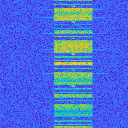
\includegraphics[width=0.14\textwidth]{img/LTE_frame_0.png} & 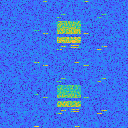
\includegraphics[width=0.14\textwidth]{img/NR_frame_1506.png} &
        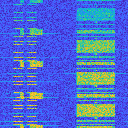
\includegraphics[width=0.14\textwidth]{img/LTE_NR_frame_0.png} & \\
        a) & b) & c)
    \end{tabular}
    \caption{spectrum samples: a) spectrum sample for LTE, b) spectrum sample for 5G NR, c) spectrum sample for overlapping 5G NR and LTE}
    \label{fig2}
\end{figure}

\subsection{WiComNet: robust and cost-efficient convolution network}
In this work, we propose the WiComNet that is a robust and cost-efficient convolution network (convnet) utilizing Unet-based architecture \cite{ronneberger2015u}. In general, this work utilizes depthwise separable convolutions (DSC) \cite{CholletXception} as convolution operation that replace for traditional convolutions. DSC uses inoperative depthwise convolution and pointwise convolution to reduce significantly the number of convolution operators. The detail of DSC can be illustrated in formula (\ref{eq:Fdsc}). Where \(F_{\text{DSC}}(f)\) denotes for the output of DSC convolution operation with the number of features extraction \(f\) , \(Dwconv(3\times3,1)_{\text{BN}}\) represents for depthwise convolution and batch normalization active function, it is connected directly by \(Conv(1\times1,f)_{\text{Relu}}\).

\begin{equation}
    F_{\text{DSC}}(f) = Dwconv(3\times3,1)_{\text{BN}} * Conv(1\times1,f)_{\text{Relu}}
    \label{eq:Fdsc}
\end{equation}

\indent On the other hand, this work applies atrous spatial pyramind pooling (ASPP) modules \cite{ChenAtrous} between encoder and decoder paths of WiComNet to enhance the ability of feature extraction in multiple scales. ASPP modules incorporate parallel four convolution layers, which include a \(1\times1\) convolution layer and three \(3\times3\) convolution layers in difference dilatation rates. The output of ASPP module is synthetic by a concatenation layer. The figure \ref{fig3} depicts ASPP module with \(r_1, r_2, r_3)\) represent for dilatation rates of three \(3\times3\) convolution layers. 

\begin{figure}[!ht]
    \centering
    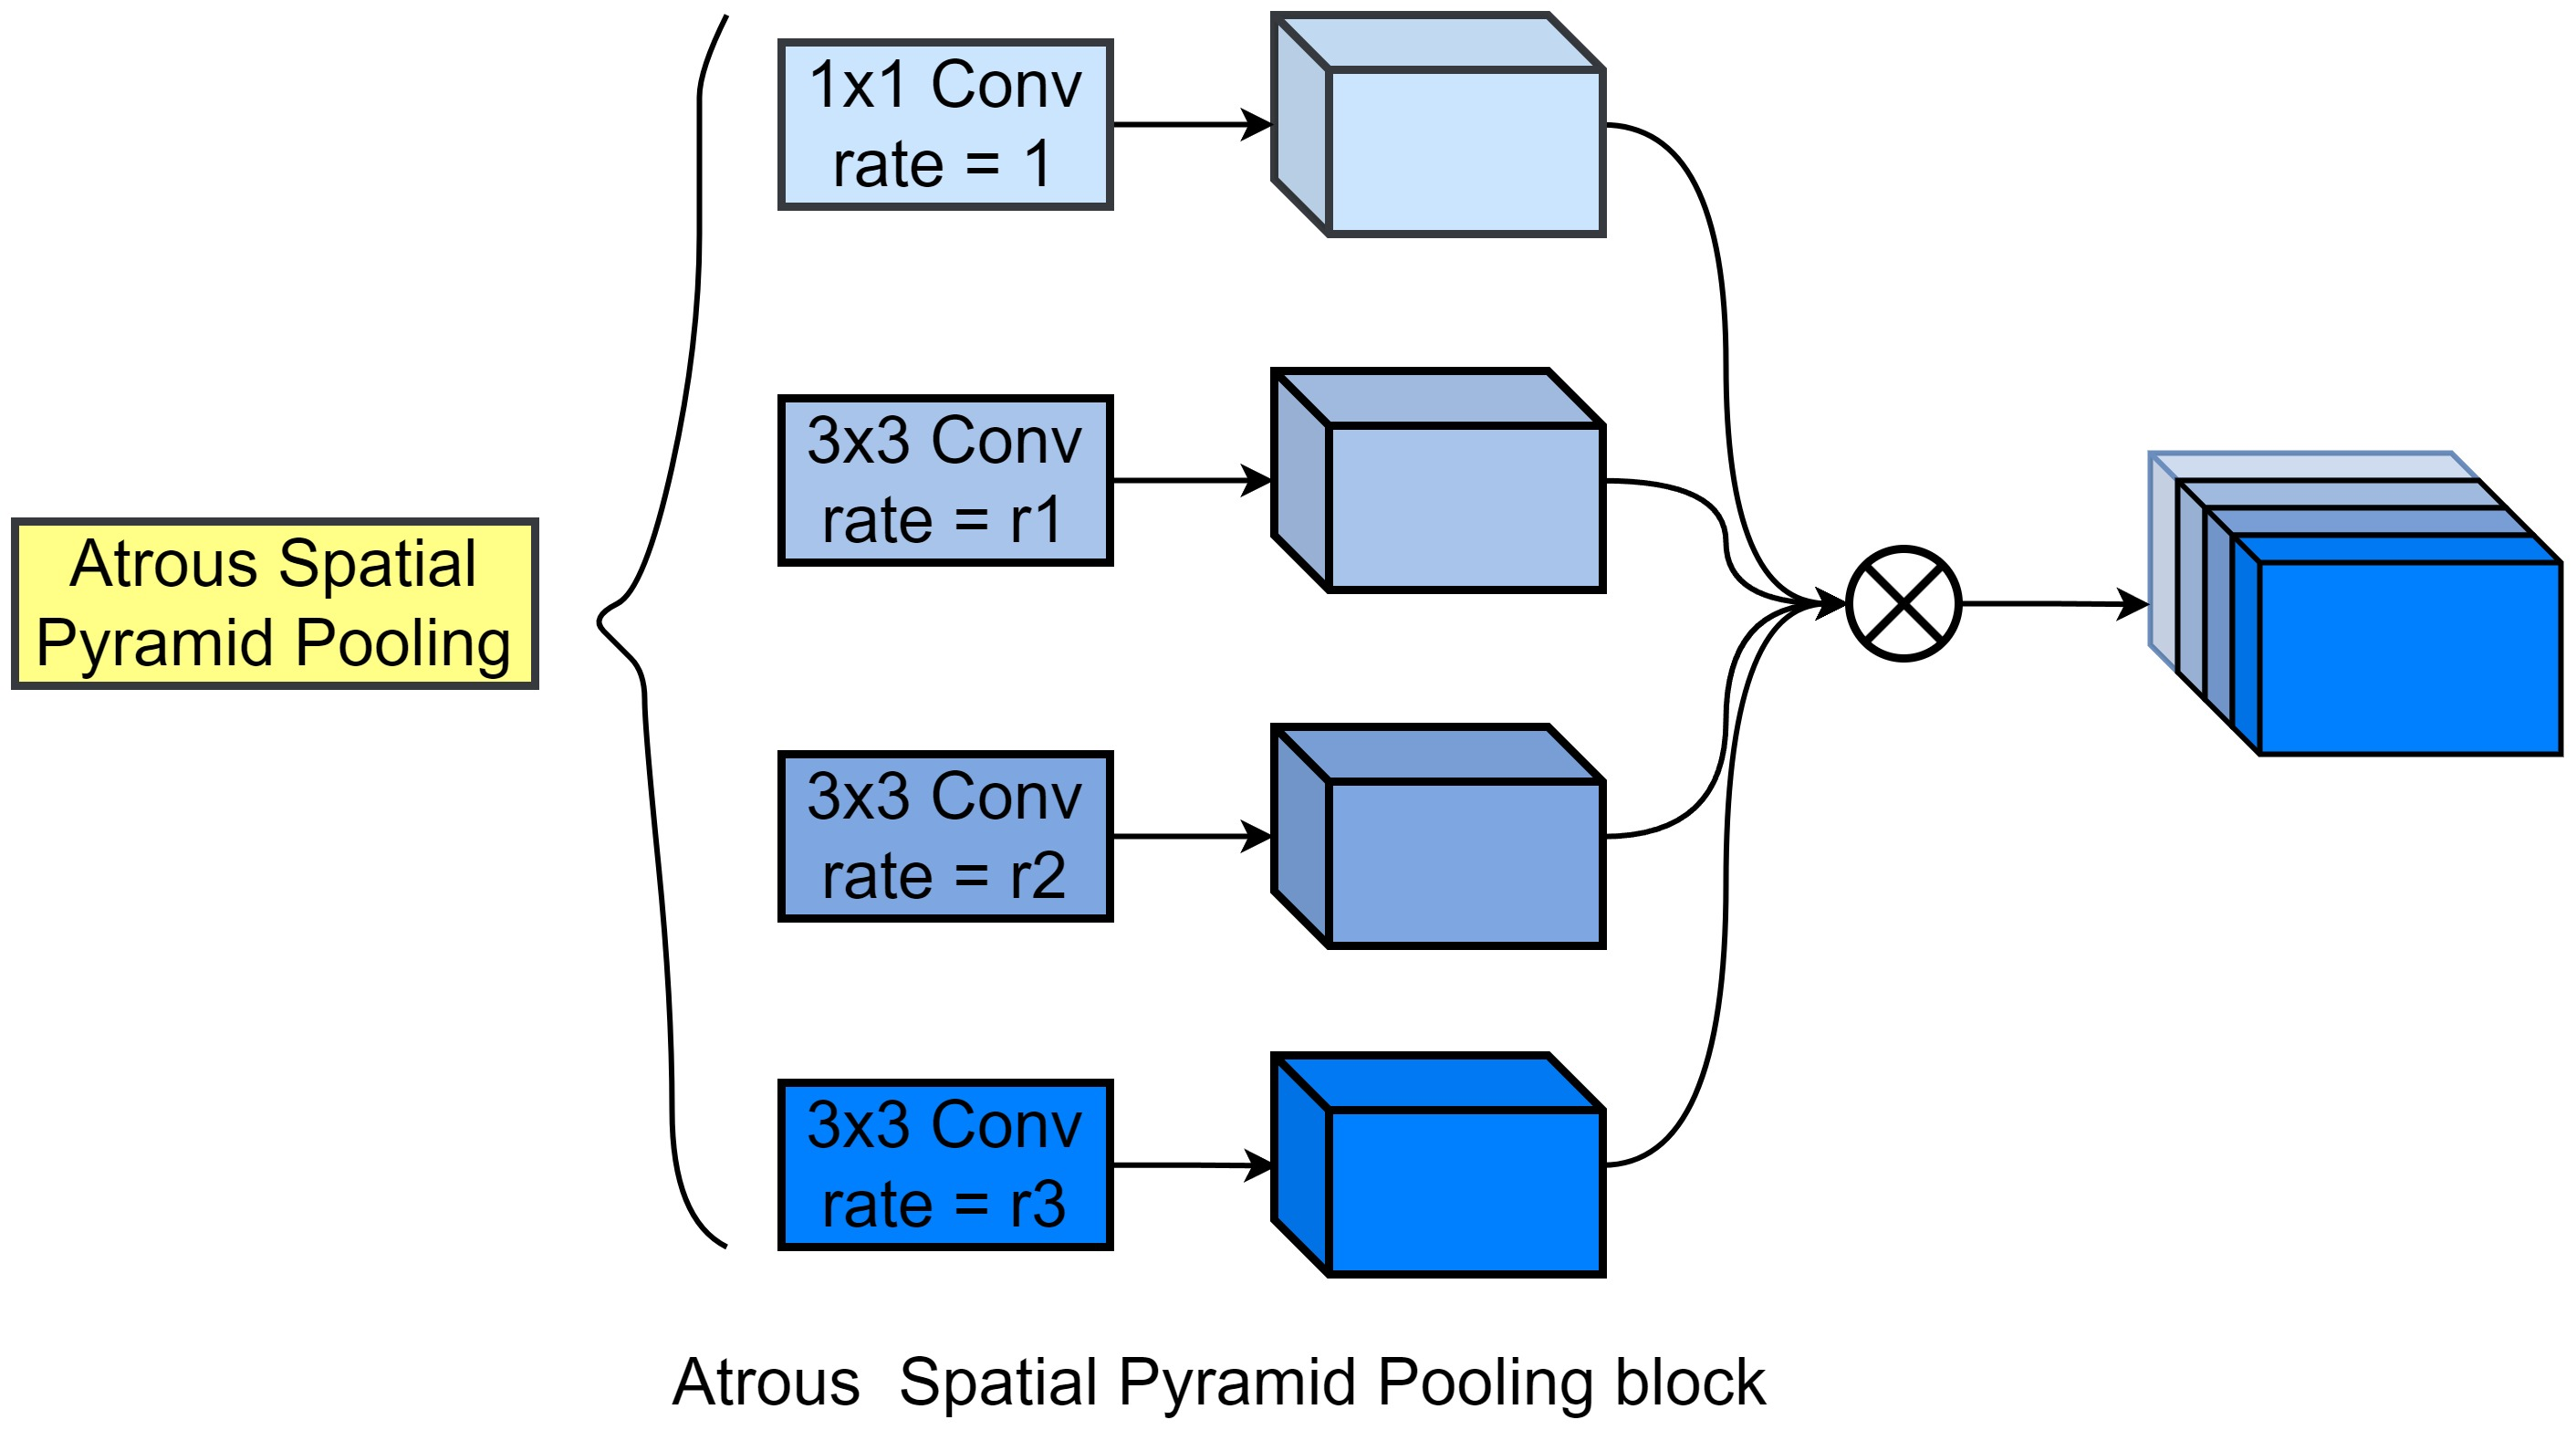
\includegraphics[width=0.35\textwidth]{img/Design-ASPP.jpg}
    \caption{Atrous spatial pyramid pooling module}
    \label{fig3}
\end{figure}

\indent The output of ASPP module can be calculated by (\ref{eq:ASPP}). Where \(F_{\text{ASPP}}(f, r_1, r_2, r_3)\) illustrates for the output of ASPP module, while \(r_1, r_2, r_3\) represents for dilatation rates, \(f\) indicates for the number of input features. Furthermore, \(F_{\text{Concat}}\) denotes for the output of concatenation operation and \(Conv\) denotes for convolution layers respectively.

\begin{equation}
\begin{aligned}
    F_{\text{ASPP}}(f,r_1,r_2,r_3) = F_{\text{Concat}}\left( Conv(1 \times 1, f),\\ 
    Conv(3 \times 3,f,r_1),   \\
    Conv(3 \times 3,f,r_2),  \\
    Conv(3 \times 3,f,r_3) \right))
    \label{eq:ASPP}
\end{aligned}
\end{equation}


\indent Inspired by the architectural innovation of the Recurrent Residual Block (RRB) as proposed in \cite{aghalari2021brain} and \cite{he2016deep}, we have revolutionized our network design. Specifically, we have overhauled both the encoder and decoder paths of our network by substituting the conventional Unet convolution blocks with RRB blocks. In WiComNet architecture, the output of each RRB block is seamlessly integrated with a cascade of DSC blocks, augmented by a residual path. This augmentation significantly amplifies the richness and complexity of the feature representation captured by our network, it is showed by figure \ref{fig4}. The formula (\ref{eq:RRB}) illustrates for the output of RRB block, \(F_{\text{add}}\) denotes for addition operation between both input \(F_{\text{in}}(f)\) and \(Conv(1\times1,f)\) from previous layer, in which \(F_{\text{in}}(f)\) is the result of previous layer, \(Conv(1\times1,f)\) and \(f\) are convolution layer and the number of input features respectively.


\begin{equation}
\begin{aligned}
    F_{\text{RRB}}(f) = F_{\text{add}}\left( F_{\text{in}}(f), Conv(1\times1,f)
    \label{eq:RRB}
\end{aligned}
\end{equation}

\begin{figure}[!ht]
    \centering
    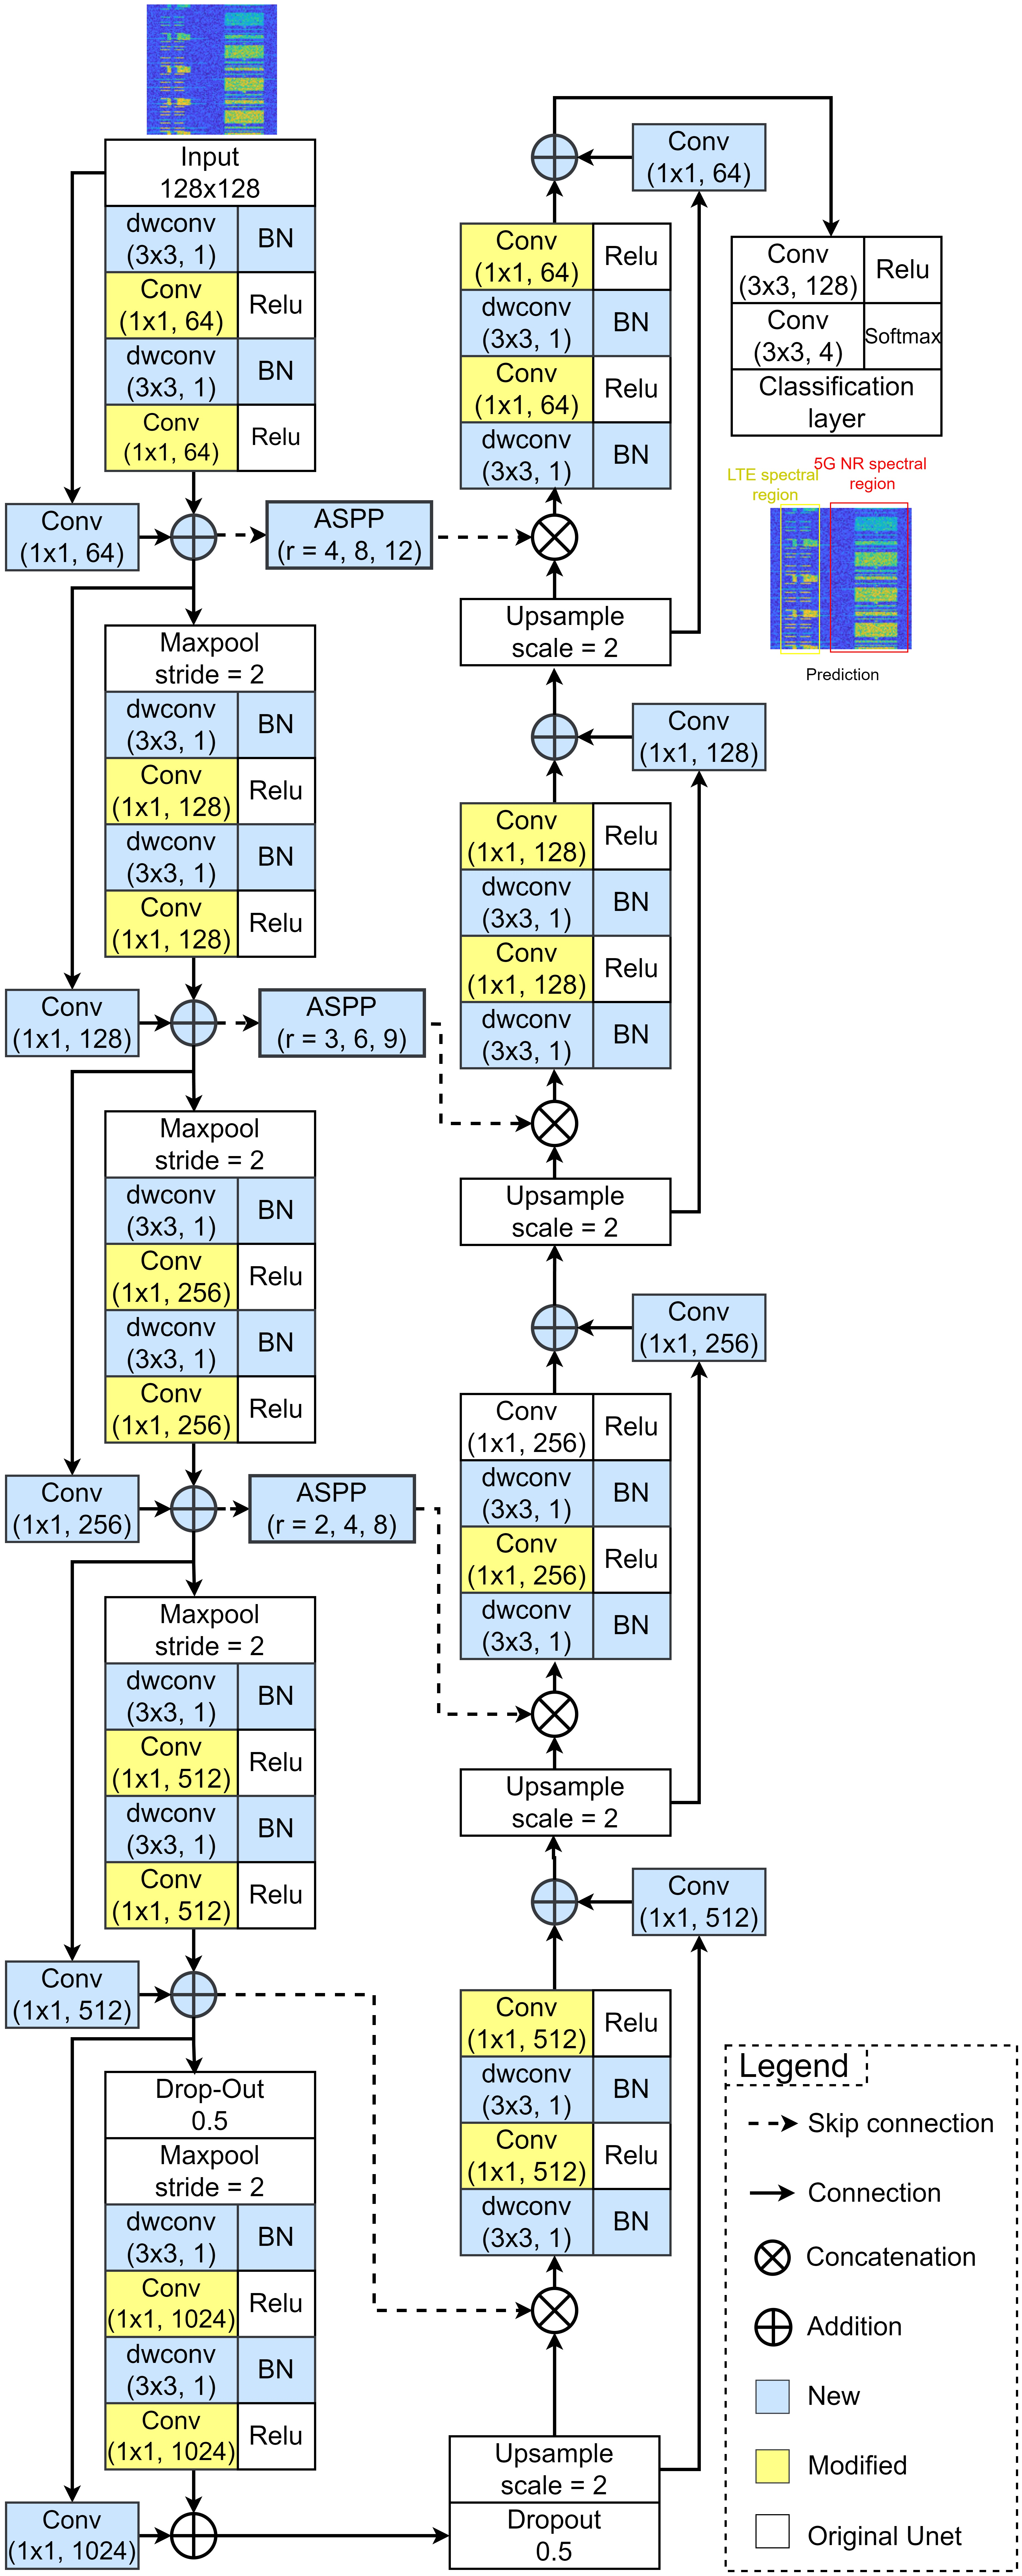
\includegraphics[width=0.35\textwidth]{img/Design-WiComNetB.jpg}
    \caption{Wireless communication network}
    \label{fig4}
\end{figure}


\indent The figure \ref{fig4} depicts for WiComNet architecture that was redesigned by Unet-based architecture \cite{ronneberger2015u}. The WiComNet architecture comprises five layers each for the encoder and decoder paths, ASPP modules are integrated into skip connection paths across multiple layers to enhance feature extraction across various scales. Our proposing design offers lowest complexity comparing to original Unet architecture, and other variants. The table \ref{tab1} compares complexities among our design with other architectures.

\begin{table}[!htbp]
\centering
\caption{Network complexity comparision}
\label{tab1}
\begin{tabular}{|c|c|c|}
\toprule
\hline
\textbf{Network} & \textbf{No. Layers} & \textbf{No. Params} \\
\hline
WiComNet & 125 & \textbf{7.8M} \\
\hline
ConvNet & 100 & 20.6M \\
\hline
Deeplabv3 & 100 & 20.6M  \\
\hline
Unet & 59 & 31.3M \\
\hline
Unetp & 101 & 42.5M  \\
\hline
UnetE & 101 & 42.3M \\
\hline
Unetpp & 101 & 43.5M  \\
\hline
\bottomrule
\end{tabular}
\end{table}



\section{Evaluation result}
\subsection{Dataset and training resource}

\subsection{WiComNet evaluation result}

\section{Conclusion}



\bibliographystyle{IEEEtran}
\bibliography{reference}

\end{document}


